\section{Remarks IBM models}

\frame[<+->]{
	\frametitle{Alignment distribution}
	Position parameterisation $L^2 \times M^2$
	Jump distribution \hfill \citep{Vogel+1996:HMMWA}
	\begin{itemize}
		\item define a jump function
		$\delta(a_j, j, l, m) = a_j - \left \lfloor j \frac{l}{m} \right \rfloor$
		\item $p(a_j|l, m) = \Cat(\Delta|\delta)$
		\item $\Delta$ takes values from $-\text{longest}$ to $+\text{longest}$ \\
		where $ \Delta = \left \langle  \delta_{-L}, ...,\delta_L \right \rangle$ is a vector of parameters called \cblue{jump probabilities}
		\item The categorical distribution  is defined for jumps ranging from $-L$ to $ L$ \\
		The jump function defines the support of the alignment distribution
		\item A jump quantifies a notion of mismatch in linear order between French and English\\
		Leads to a very small number of parameters, $2 \times L$
	\end{itemize}
}

\frame{
	\frametitle{IBM 2 EM}
	
	\begin{figure}
		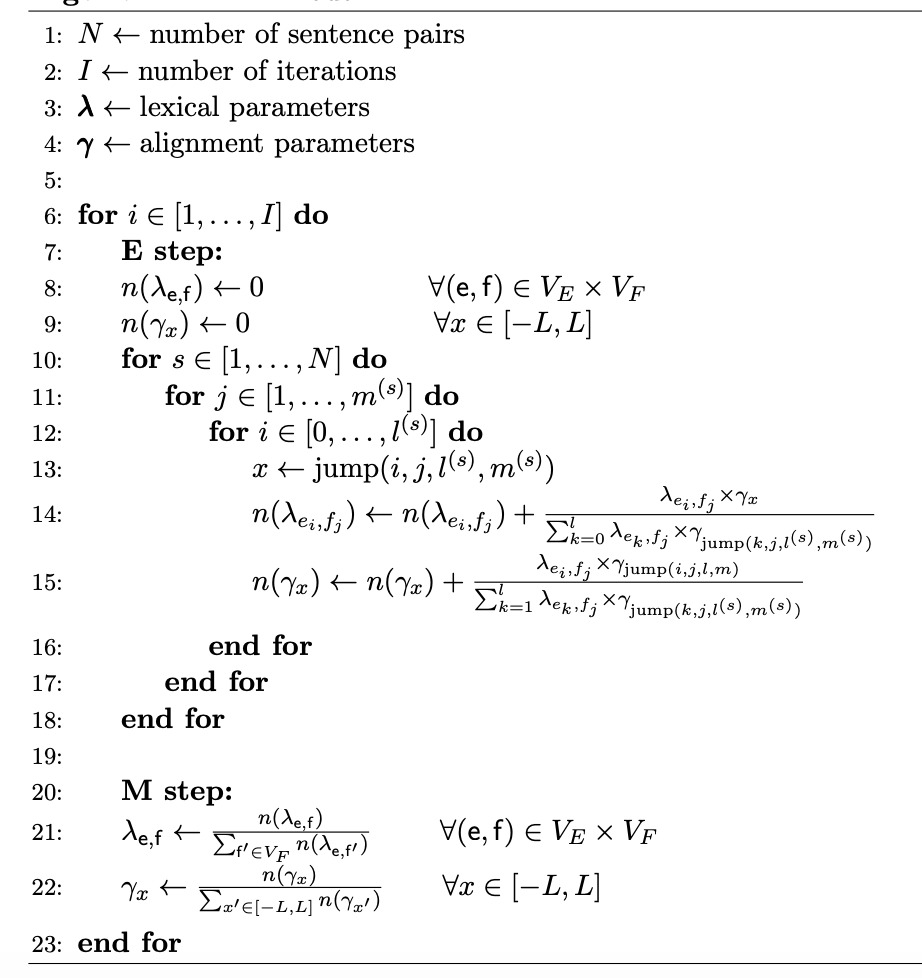
\includegraphics[scale=0.5]{ibm2_algo}
		\end{figure}
	
}


\frame[<+->]{
	\frametitle{EM non identifiability}
	
	IBM 1
	\begin{itemize}
		\item The mixture weights are fixed and uniform, \\
		EM is guaranteed to arrive at a \cblue{global maximum}.
		\item But there may be local maxima
		\item  It is not strictly convex, where multiple parameter settings that achieve the same global optima
		\item  The possible MLEs the EM algorithm finds depends on the \cblue{starting parameters}
		\item In practice, one usually starts from uniform parameters. \\
		\citep{Toutanova+2011:IBM1} show better initialisations
		
	\end{itemize}
	
}


\frame[<+->]{
	\frametitle{EM non identifiability}
	
	IBM 2
	\begin{itemize}
		\item Mixture weights are not fixed and we  add several new parameters \\
		 Given  asymmetric mixture weights, most maxima are now local.
		 \item Mixture weights are not uniform\\
		 No guaranteed to be a global maximum. 
		 \item Changing weights may change in the component distributions and the other way around.
		 \item  In practice, one initialises the component distributions of IBM2 (i.e. its translation parameters) with IBM1 estimates. 
		 \item The alignment distributions are initialised uniformly. Notice we first have to train IBM1 before proceeding to IBM2
		
		
	\end{itemize}
	
}


\section{Representation}

\frame{
	\frametitle{IBM 1-2: strong assumptions}
	
	Independence assumptions
	\begin{itemize}
		\item $p(a|m, n)$ does not depend on lexical choices\\
		a$_1$ \textcolor{red}{cute}$_2$ house$_3$ $\leftrightarrow$ una$_1$  casa$_3$  \textcolor{red}{bella}$_2$\\ \pause
		a$_1$ \textcolor{blue}{cosy}$_2$ house$_3$ $\leftrightarrow$ una$_1$ casa$_3$ \textcolor{blue}{confortable}$_2$ \\ \pause
		\item $p(f|e)$ can only reasonably explain one-to-one alignments\\		
		I \alert{will be leaving} \textcolor{blue}{soon} $\leftrightarrow$ \alert{voy a salir} \textcolor{blue}{pronto} \pause
	\end{itemize}
	
	~ 
	
	Parameterisation
	\begin{itemize}
		\item categorical events are unrelated \\
		prefixes/suffixes: normal, normally, abnormally, $\ldots$\\
		verb inflections: comer, comi, comia, comio, $\ldots$ \\
		gender/number: gato, gatos, gata, gatas, $\ldots$ 
		%\item number of parameters grows with data\\
		%$P(F|E)$ takes $O(v_F \times v_E)$ parameters
	\end{itemize}
	
}

\frame[<+->]{
	\frametitle{Conditional probability distributions}
	
	CPD: condition $c \in \mathcal C$, outcome $o \in \mathcal O$, and $\theta_{c} \in \mathbb R^{|\mathcal O|}$
	\begin{center}
	\begin{align}
		p(o|c) &= \Cat(\theta_c)  
	\end{align}
	\end{center}
	\begin{itemize}
		\item $p(o|c) = \theta_{c, o}$
		\item $0 \le \theta_{c, o} \le 1$
		\item $\sum_o \theta_{c, o} = 1$
		\item $O(|\mathcal c| \times |\mathcal o|)$ parameters
	\end{itemize}
	
	~
	
	\hfill \alert{How bad is it for IBM model 1?}
}

\frame{
	\frametitle{Probability tables}
	
	\begin{center}
	$$p(f|e)$$
	\begin{tabular}{| l | l | l | l | l |} \hline
	\multirow{2}{*}{\sc English $\downarrow$} & \multicolumn{4}{c|}{\sc French $\rightarrow$} \\ \cline{2-5}
	         & anormal & normal & normalmente & $\ldots$ \\ \hline
	abnormal & 0.7     & 0.1    & 0.01        & $\ldots$ \\ \hline
	normal   & 0.01    & 0.6    & 0.2         & $\ldots$ \\ \hline
	normally & 0.001   & 0.25   & 0.65        & $\ldots$ \\ \hline	
	\end{tabular}
	\end{center}
	
	\begin{itemize}
		\item grows with size of vocabularies
		\item no parameter sharing
	\end{itemize}
}

\frame{
	\frametitle{Logistic CPDs}
	
	CPD: condition $c \in \mathcal C$ and outcome $o \in \mathcal O$
	\begin{center}
	\begin{align}
		p(o|c) &= \frac{\exp(w^\top h(c, o))}{\sum_{o'} \exp(w^\top h(c, o'))} 
	\end{align}
	\end{center}
	\begin{itemize}
		\item $w \in \mathbb R^d$ is a weight vector
		\item $h: \mathcal C \times \mathcal O \rightarrow R^d$ is a feature function
		\item $d$ parameters
		\item computing CPD requires $O(|\mathcal c| \times |\mathcal o| \times d)$ operations
	\end{itemize}
	
	~
	
	\hfill \alert{How bad is it for IBM model 1?}
}


\frame{
	\frametitle{CPDs as functions}
	
	\begin{center}
	\begin{footnotesize}
	$$h: \mathcal E \times \mathcal F \rightarrow R^d$$
	\begin{tabular}{|l | l | l | l | l | l|l|} \hline
	\multicolumn{2}{|c|}{\sc Events $\downarrow$} & 
	\multicolumn{5}{c|}{\sc Features $\rightarrow$} \\ \hline
	\multirow{2}{*}{\sc English} & 
	\multirow{2}{*}{\sc French} & 
		{\bf normal} & \emph{normal-} & \underline{-normal} & \alert{ab-} & \textcolor{blue}{-ly}  \\
		& & {\bf normal} & \emph{normal-}& \underline{-normal} & \alert{a-} & \textcolor{blue}{-mente} \\ \hline \hline
	% ABNORMAL
	\multirow{3}{*}{abnormal} & \alert{a}\underline{normal} & 0 & 0 & 1 & 1 & 0 \\ \cline{2-7}
	             & \underline{normal} & 0 & 0 & 1 & 0 & 0 \\ \cline{2-7}
	             & \textit{normal}mente & 0 & 1 & 0 & 0 & 0 \\ \hline \hline
	% NORMAL
	\multirow{3}{*}{normal} 
	             & a\underline{normal}       & 0 & 0 & 1 & 0 & 0 \\ \cline{2-7}
	             & {\bf normal}  & 1 & 0 & 0 & 0 & 0 \\ \cline{2-7}
	             & \emph{normal}mente   & 0 & 1 & 0 & 0 & 0 \\ \hline \hline	
	% NORMALLY
	\multirow{3}{*}{normally} 
	             & a\underline{normal}       & 0 & 0 & 1 & 0 & 0 \\ \cline{2-7}
	             & \textit{normal}  & 0 & 1 & 0 & 0 & 0 \\ \cline{2-7}
	             & \emph{normal}\textcolor{blue}{mente}   & 0 & 1 & 0 & 0 & 1 \\ \hline \hline	
	\multicolumn{2}{|c|}{\sc Weights $\rightarrow$} & 1.5 & 0.3 & 0.3 & 0.8 & 1.1 \\ \hline
	\end{tabular}
	\end{footnotesize}
	\end{center}
	
	\begin{itemize}
		\item computation still grows with size of vocabularies
		\item but far less parameters to estimate
	\end{itemize}
}



\section{Feature rich models}

\frame[<+->]{
	\frametitle{Log-linear models}
	\begin{itemize}
	\item Log-linear models revolve around the concept of features. In short, features are basically,\\
	 Something about the context that will be useful in predicting
	\item Enhancing models with \cblue{features} that capture the dependencies between different morphologically inflected word forms.
The standard parameterisation using categorical distributions is limited with respect to the features it can capture
	
	\end{itemize}
	
	
}


%\frame[<+->]{
%	\frametitle{Log-linear models}
%	\begin{itemize}
%	\item 
%	\end{itemize}
	
	
%}


\section{Feature-rich IBM 1-2}

\frame{
	\frametitle{\citet{Berg+2010:PU}}
	
	Lexical distribution in IBM model 1
	\begin{align}
		p(f|e) &= \frac{\exp(w_{\text{lex}}^\top h_{\text{lex}}(e, f))}{\sum_{f'} \exp(w_{\text{lex}}^\top h_{\text{lex}}(e, f'))} 
	\end{align}
	
	~
	
	Features
	\begin{itemize}
		\item $f \in V_F$ is a French word (decision), $e \in V_E$ is an English word (conditioning context), 
				$w \in R^d$ is the parameter vector, and $h : V_F × V_E \rightarrow R^d$ is a feature vector function.
		\item prefixes/suffixes
		\item character $n$-grams
		\item POS tags
	\end{itemize}

}

\frame{
	\frametitle{Extension: lexicalised jump distribution}

	\begin{align}
		p(\delta|e) &= \frac{\exp(w_{\text{dist}}^\top h_{\text{dist}}(e, \delta))}{\sum_{\delta'} \exp(w_{\text{dist}}^\top h_{\text{dist}}(e, \delta'))} 
	\end{align}
	
	~
	
	Features
	\begin{itemize}
		\item POS tags
		\item suffixes/prefixes
		\item lemma
		\item jump values
		\item $m, n, j, i$ (values used to compute jump)
		\begin{figure}
		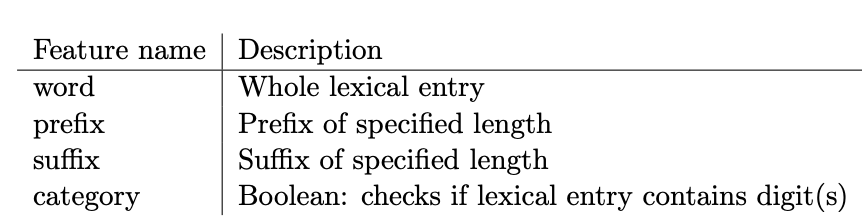
\includegraphics[scale=0.5]{feat_eg}
		\end{figure}
	\end{itemize}
}



\frame[<+->]{
	\frametitle{Problems with features}
	\begin{itemize}
	\item We can see $e_{t-2}$ = farmers is compatible with $e_t$ = hay (in the context \cblue{farmers grow hay}) 
	\item and $e_{t-1}$ = eat is also compatible (in the context \cblue{cows eat hay}).
	\begin{figure}
		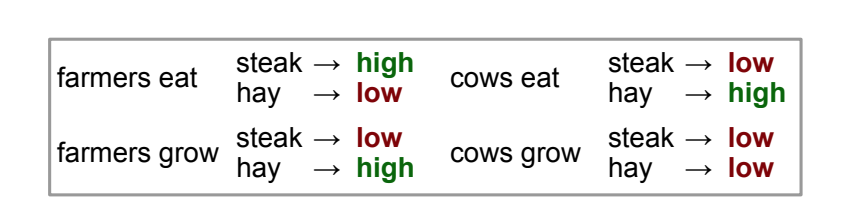
\includegraphics[scale=0.5]{feat_problem}
	\end{figure}
	\end{itemize}
	
	
}

\frame[<+->]{
	\frametitle{Problems with features}
	\begin{itemize}
	
	\item Features depend on $e_{t-1}$, and another set of features dependent on $e_{t-2}$, neither set of features can rule out
	the unnatural phrase \cred{farmers eat hay}
	\item Combination of features greatly expands the parameters: instead of $O(|V |^2)$ parameters for each pair $e_{i-1}$, $e_i$,\\
	 We need $O(|V |^3)$ parameters for each triplet $e_{i-2}, e_{i-1}, e_i$
	\item Learning using these combination features, e.g. \cblue{neural networks}
	\end{itemize}
	
	
}

\section{Overview of Neural Networks}

\frame[<+->]{
	\frametitle{Function that cannot be solved by a linear transformation}
	\begin{itemize}
	\item For example the function  $x \in {-1, 1}$ and outputs $y = 1$ \\
	 if both $x_1$ and $x_2$ are equal and $y = -1$ otherwise.
	 \begin{figure}
		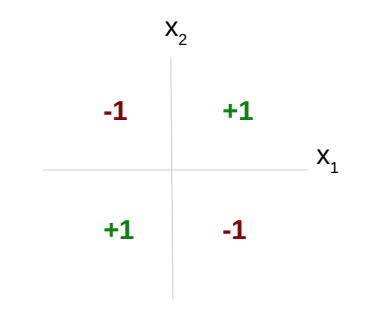
\includegraphics[scale=0.5]{nonlinear_func}
	\end{figure}
	 \item We can use a linear combination $y = Wx + b$
	 \item Or a multi-layer perceptron:
	 \begin{equation}
	 \begin{aligned}
	 h & = step(W_x h_x + b_h) \\
	y & = w_{hy} h + b_y.
	 \end{aligned}
\end{equation}	  

	\end{itemize}
	
	
}


\frame[<+->]{
	\frametitle{Function that cannot be solved by a linear transformation}
	\begin{itemize}
	
	\item Computation is split into two stages: 
	\item Calculation of the hidden layer , which takes in input
	$x$ and outputs a vector of hidden variables $h$
 	\item and calculation of the output layer, which
		takes in $h$ and calculates the final result $y$. 
	\item Both layers consist of an affine transform
	using weights $W$ and biases $b$, followed by a $step(·)$ function, which calculates the following:
	\begin{equation}
	\begin{aligned}
	step(x)=\begin{cases}
    		1, & \text{if }x > 0. \\
    		-1, & \text{otherwise}.
	\end{cases} 
	\end{aligned}
	\end{equation}
	\item 
	 \begin{figure}
		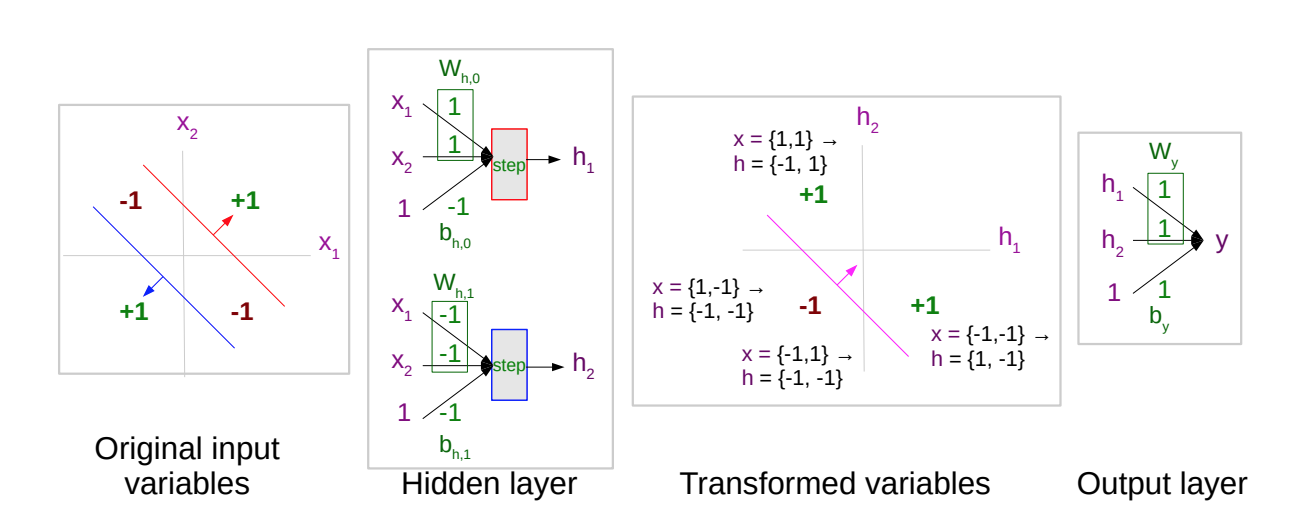
\includegraphics[scale=0.35]{nonlinear_mlp}
	\end{figure}
	\end{itemize}
	
	
}




\frame[<+->]{
	\frametitle{Training Neural Networks}
	\begin{itemize}
	\item  We would like to train the parameters of the MLP
	\item We need to define the loss function $ l(·)$, calculate the derivative of the loss with respect to the
parameters, then take a step in the direction that will reduce the loss.
	\item e.g. squared-error loss, common in regression problems\\
which measures the difference between the calculated value $y$ and correct value $y^*$:\\
	$l(y^*, y) = (y^* - y)^2$
	\item however the $step()$ function is  not very derivative friendly
	\item We can use non-linear functions,  hyperbolic	tangent (\cblue{tanh}) function
	 \begin{figure}
		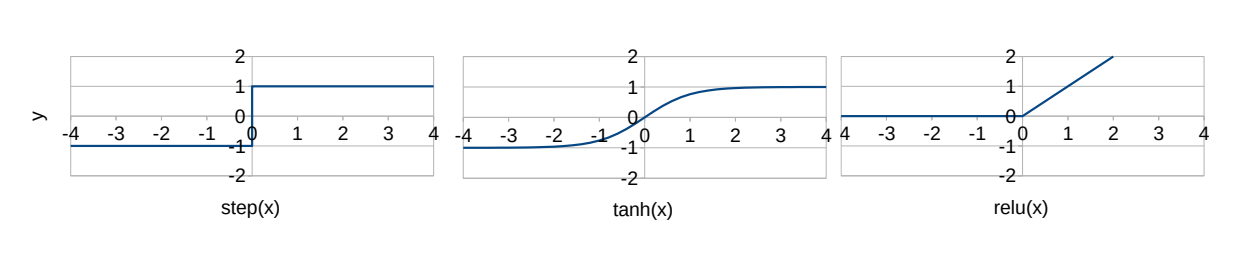
\includegraphics[scale=0.45]{nonlinearities}
	\end{figure}
	\end{itemize}
	
	
}


\frame[<+->]{
	\frametitle{Training Neural Networks}
	\begin{itemize}
	\item   We perform the full calculation of the loss function:
	\begin{figure}
		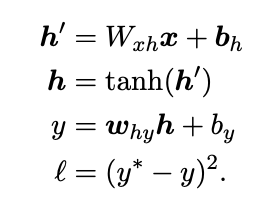
\includegraphics[scale=0.45]{nonlinear_tanh}
	\end{figure}
	\item Computation graph:
	\begin{figure}
		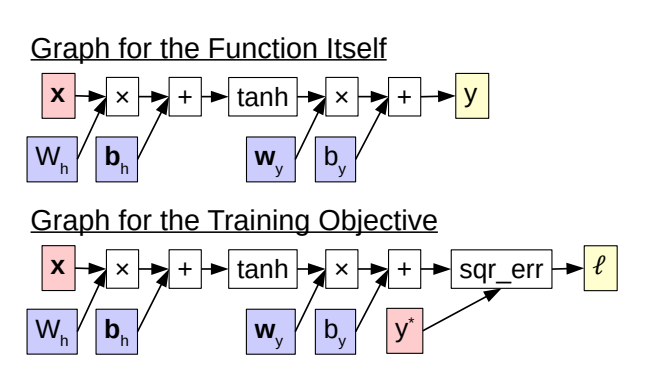
\includegraphics[scale=0.30]{comp_graph}
	\end{figure}
	\item   We use chain rule of derivatives for each set of parameters:
	\begin{figure}
		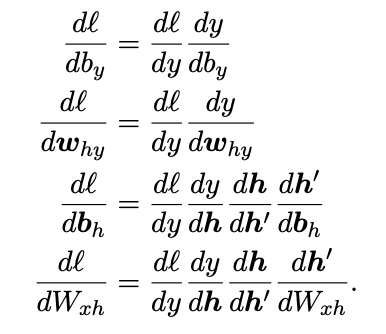
\includegraphics[scale=0.45]{nonlinear_diff}
	\end{figure}
	\item 
	\end{itemize}
	
	
}

\section{Neural  IBM 1}

\frame[<+->]{
	\frametitle{IBM: non-linear models}
	
	Nothing prevents us from using more expressive functions \\
	\hfill \citep{Kovcisky+2014:NIBM}
	\begin{itemize}		
		\item $p(o|c) = \softmax(f_\theta(c))$
		\item $p(o|c) = \frac{\exp(f_\theta(c, o)))}{\sum_{o'} \exp(f_\theta(c, o')))}$
	\end{itemize}
	
	~ where $f_\theta(\cdot)$ is a neural network with parameters $\theta$ 
	
	Features
	\begin{itemize}
		\item induce features (word-level, char-level, $n$-gram level)
		\item pre-trained embeddings
	\end{itemize}
	
}

\frame[<+->]{
	\frametitle{Neural IBM}
	\begin{itemize}
	\item  $f_\theta(e) = \mathrm{softmax}(W_t H_E(e) + b_t)$
note that the softmax is necessary to make $t_\theta$ produce valid parameters for the categorical distribution \\
$W_t \in \mathbb R^{|V_F| \times d_h}$ and $b_t \in \mathbb R^{|V_F|}$ 


	\end{itemize}


 
}


\frame[<+->]{
	\frametitle{Neural IBM}
	\begin{itemize}
	
\item $h_E(e)$ is defined below with $W_{h_E} \in \mathbb R^{d_h \times d_e}$ and $b_{h_E} \in \mathbb R^{d_h}$  \\
 $ h_E(e) = \underbrace{\tanh(\underbrace{W_{h_E} r_E(e) + b_{h_E}}_{\text{affine}})}_{\text{elementwise nonlinearity}}$ 
\item $r_E(e) = W_{r_E} v_E(e)$ is a word embedding of $e$ with $W_{r_E} \in \mathbb R^{d_e \times |V_E|}$ 
\item $v_E(e) \in \{0,1\}^{v_E} $ is a one-hot encoding of $e$, thus $\sum_i v_E(e)_i = 1$ 
\item $\theta = \{W_t, b_t, W_{h_E}, b_{h_E}, W_{r_E}\}$
\item Other architectures are also possible, one can use different parameterisations that may use more or less parameters. For example, with a CNN one could make this function sensitive to characters in the words, something along these lines could also be done with RNNs.
	\end{itemize}
	where

 
}

\frame[<+->]{
	\frametitle{MLE}
	\begin{itemize}
	\item We can use maximum likelihood estimation (MLE) to choose the parameters of our deterministic function $f_\theta$. 
	\item We know at least one general (convex) optimisation algorithm, i.e. gradient ascent. \\
	 This is a gradient-based procedure which chooses $\theta$ so that the gradient of our objective with respect to $\theta$ is zero. 
	 \item  IBM1 would be convex with standard tabular CPDs, but FFNNs with 1 non-linear hidden layer (or more) make it non-convex.

	\item Nowadays, we have tools that can perform automatic differentiation for us. \\
	If our functions are differentiable, we can get gradients for them.

	\end{itemize}
}


\frame[<+->]{
	\frametitle{MLE}
	\begin{itemize}


	\item We still need to be able to express the functional form of the likelihood.

	
	\item  Let us then express the log-likelihood (which is the objective we maximise in MLE) of a single sentence pair as a function of our free parameters:
	\begin{equation}
	\begin{aligned}
    \mathcal L(\theta|e_0^m, f_1^n) = \log p_\theta(f_1^m|e_0^l) 
    \end{aligned}
	\end{equation}


	\item Note that in fact our log-likelihood is a sum of independent terms $\mathcal L_j(\theta|e_0^m, f_j)$, thus we can characterise the contribution of each French word in each sentence pair as




	\end{itemize}
}

\frame[<+->]{
	\frametitle{MLE}
	
	\begin{itemize}
	\item  NN toolkits implement gradient-based optimisation for us. 
	\item  To get a loss, we simply negate our objective. \\
	You will find a lot of material that mentions some categorical cross-entropy loss.
	\begin{equation}
	\begin{aligned}
    l(\theta) & = -\sum_{(e_0^m, f_1^l)} p_\star(f_1^l|e_0^m) \log p_\theta(f_1^m|e_0^l) \\
     & \approx -\frac{1}{S} \log p_\theta(f_1^l|e_0^m)
\end{aligned}
	\end{equation}

	\end{itemize}

}


\frame[<+->]{
	\frametitle{MLE}
	
	\begin{itemize}
	
	\item With SGD we sample a subset $\mathcal S$ of the training data and compute a loss for that sample. 
	\item We then use automatic differentiation to obtain a gradient $\nabla_\theta \mathcal l(\theta|\mathcal S)$. This gradient is used to update our deterministic parameters $\theta$.
	\begin{equation}
	\begin{aligned}
	\theta^{(t+1)} = \theta^{(t)} - \delta_t \nabla_{\theta^{(t)}} l(\theta^{(t)}|\mathcal S)
	\end{aligned}
	\end{equation}
	
	\end{itemize}

}

